%%%%%%%%%%%%%%%%%%%%%%%%%%%%%%%%%%%%%%%%%%%%%%%%%%%%%%%%%%%%%%%%%
\section{Thermodynamics}
%%%%%%%%%%%%%%%%%%%%%%%%%%%%%%%%%%%%%%%%%%%%%%%%%%%%%%%%%%%%%%%%%
In the previous sections, we already used basic concepts of gas dynamics to derive the thrust equation. Here, we review all essential gas-dynamic and thermodynamic concepts that we need for the gas turbine cycle analysis.
%%%%%%%%%%%%%%%%%%%%%%%%%%%%%%%%%%%%%%%%%%%%%%%%%%%%%%%%%%%%%%%%%
\subsection{Conservation Equations}
%%%%%%%%%%%%%%%%%%%%%%%%%%%%%%%%%%%%%%%%%%%%%%%%%%%%%%%%%%%%%%%%%
Recall the general form of a conservation equation of any quantity $\phi = \{{\text{mass},\, \text{momentum},\, \text{energy}}$\},
\begin{equation}
\text{accumulation}(\phi) + \text{outflow}(\phi) - \text{inflow}(\phi) = \text{production}(\phi)\,.
\end{equation}
For the following analysis, we will consider a control volume analysis, which is illustrated in \cref{FIG_CONTROL_VOLUME}.

%================================================================
\begin{figure}[!hbt!]
  \begin{center}
    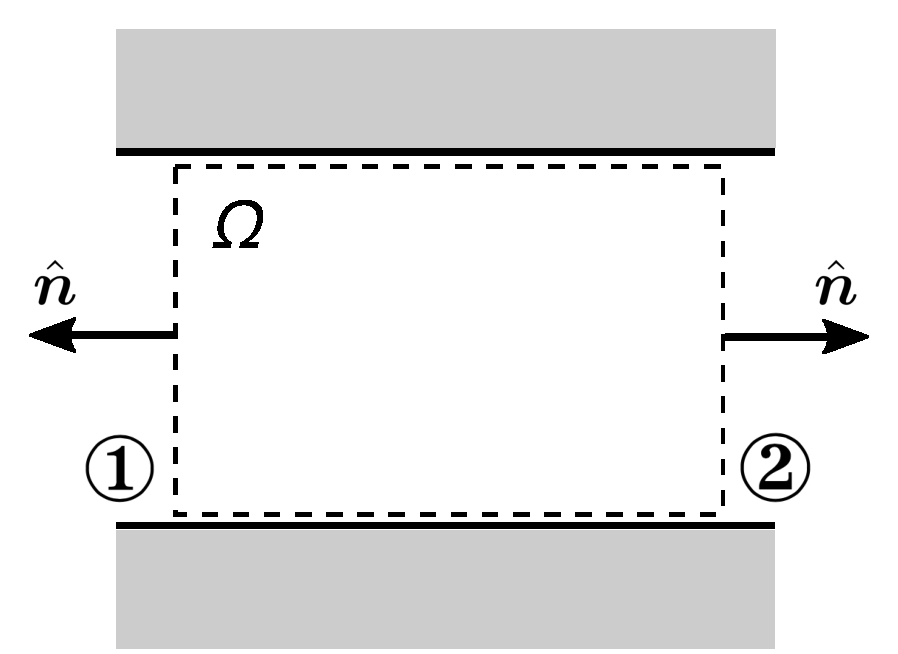
\includegraphics[width=0.38\textwidth]{ControlVolume}
    \caption{\label{FIG_CONTROL_VOLUME}Control volume.}
  \end{center}
\end{figure}
%================================================================

%%%%%%%%%%%%%%%%%%%%%%%%%%%%%%%%%%%%%%%%%%%%%%%%%%%%%%%%%%%%%%%%%
\subsubsection{Mass Conservation}
%%%%%%%%%%%%%%%%%%%%%%%%%%%%%%%%%%%%%%%%%%%%%%%%%%%%%%%%%%%%%%%%%
The governing equation describing conservation of mass can be written in the following form:
\begin{equation}
  \f{dm}{dt} = \dot{m}_\text{in} - \dot{m}_\text{out} = - \oint \rho \uvec \cdot \hat{\nvec} dA\,,
\end{equation}
where $\dot{m} = \int \rho u_\perp dA$, in which $u_\perp$ is the velocity component normal to the area $A$. For stationary flows, $dm/dt = 0$, and hence we have $\dot{m}_\text{in} = \dot{m}_\text{out}$, or
\begin{equation}
  \rho_1 u_{\perp1} A_1 = \rho_2 u_{\perp2} A_2\,,
\end{equation}
which is called the one-dimensional mass-flow equation.

%%%%%%%%%%%%%%%%%%%%%%%%%%%%%%%%%%%%%%%%%%%%%%%%%%%%%%%%%%%%%%%%%
\subsubsection{Momentum Conservation}
%%%%%%%%%%%%%%%%%%%%%%%%%%%%%%%%%%%%%%%%%%%%%%%%%%%%%%%%%%%%%%%%%
The governing equation describing conservation of momentum conservation takes the following form:
\begin{equation}
  \begin{split}
    \f{d(m \uvec)}{dt} = \f{d}{dt} \int \rho\uvec dV &= \dot{M}_\text{in} - \dot{M}_\text{out} + \sum_i \Fvec_i \\
                         &= - \oint (\rho \uvec)( \uvec \cdot \hat{\nvec}) dA + \sum_i \Fvec_i\,,
  \end{split}
\end{equation}
which is a vector equation for each velocity component $\uvec=(u_1, u_2,\ldots)^T\in\mathbb{R}^{N_d}$ (with $N_d$ being the spatial dimension). The force terms on the right-hand side are:
\begin{itemizePacked}
  \item Pressure force: $\Fvec_p = -\int \nabla p dV$;
  \item Viscous force: $\Fvec_v = -\oint \hat{\nvec} \cdot \sigmamat dA$;
  \item Gravitational force: $\Fvec_g = \int \rho \gvec dV$.
%  \item Reaction force: $\Fvec_p = -\int \nabla p dV$.
\end{itemizePacked}
Under the assumption of steady-state, the momentum conservation equation reduces to:
\begin{equation}
  \dot{M}_\text{in} - \dot{M}_\text{out}  = -\sum_i \Fvec_i\,,
\end{equation}
or for one-dimensional flows:
\begin{equation}
  (\rho_2 u_{\perp2} A_2)u_{\perp2}-(\rho_1 u_{\perp1} A_1)u_{\perp1} = p_1A_1-p_2A_2-F_D\,,
\end{equation}
where $F_D$ is the drag force, as shown in \cref{FIG_MOMENTUM_CONSERVATION}.

%================================================================
\begin{figure}[!h!]
  \begin{center}
    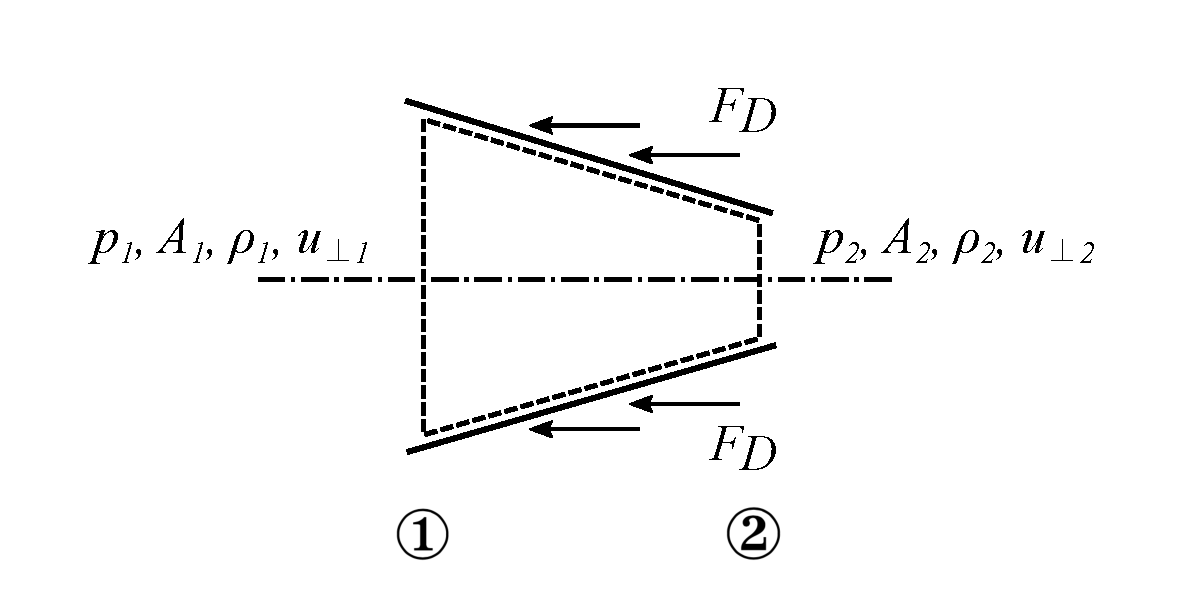
\includegraphics[width=0.65\textwidth]{MomentumConservation}
    \caption{\label{FIG_MOMENTUM_CONSERVATION}Momentum balance on control volume.}
  \end{center}
\end{figure}
%================================================================

%%%%%%%%%%%%%%%%%%%%%%%%%%%%%%%%%%%%%%%%%%%%%%%%%%%%%%%%%%%%%%%%%
\subsubsection{Energy Conservation}
%%%%%%%%%%%%%%%%%%%%%%%%%%%%%%%%%%%%%%%%%%%%%%%%%%%%%%%%%%%%%%%%%
We define the total energy as $H_T = H + \f{1}{2}m\uvec^2+mgz$ or in mass-specific form
\begin{equation}
h_T = h + \f{1}{2} u^2 + gz = h_0 + gz\,.
\end{equation}
The conservation equation is
\begin{equation}
  \f{d}{dt} \int \rho h_T dV + \oint \rho h_T (\uvec \cdot \hat{\nvec})dA =  \underbrace{\int \dot{Q} dV}_\text{Heat transfer rate}+\underbrace{\f{d}{dt}\int p dV}_\text{Technical work}+\underbrace{\int F_\sigma dV}_\text{Viscous force}\,,
\end{equation}
where $\dot{q}$ is the heat transfer rate (per unit time and unit volume). Using Fourier's law, $\dot{q}$ can be written as $\dot{q} = \nabla \cdot (\lambda \nabla T)$), and $F_\sigma = \nabla \cdot (\sigmamat \cdot \uvec)$ is the viscous dissipation.

%================================================================
\begin{figure}[!h!]
  \begin{center}
    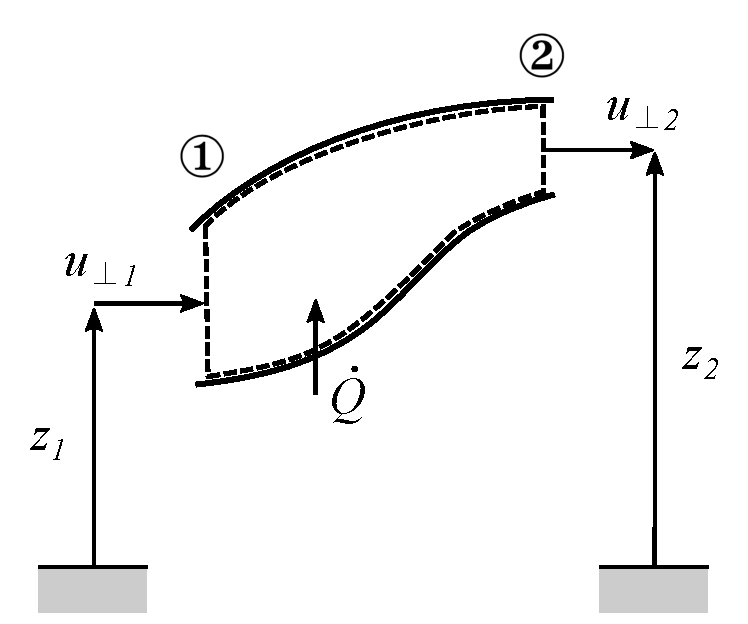
\includegraphics[width=0.52\textwidth]{EnergyConservation}
    \caption{\label{FIG_ENERGY_CONSERVATION}Control volume balance for energy equation.}
  \end{center}
\end{figure}
%================================================================

%%%%%%%%%%%%%%%%%%%%%%%%%%%%%%%%%%%%%%%%%%%%%%%%%%%%%%%%%%%%%%%%%
\subsubsection{Summary of Governing Equations}
%%%%%%%%%%%%%%%%%%%%%%%%%%%%%%%%%%%%%%%%%%%%%%%%%%%%%%%%%%%%%%%%%
In the following, we summarize the set of working equations in differential form that we will use for the subsequent analysis:
\begin{itemizePacked}
  \item Mass conservation: 
    \begin{equation}
      \partial_t \rho + \nabla \cdot (\rho \uvec) = 0\,;
    \end{equation}
  \item Momentum conservation: 
    \begin{equation}
      \partial_t (\rho \uvec) + \nabla \cdot (\rho \uvec \otimes \uvec) = - \nabla p + \nabla \cdot \sigmamat\,;
    \end{equation}
  \item Energy conservation: 
    \begin{equation}
      \partial_t (\rho h_T) + \nabla \cdot (\rho \uvec h_T) = \partial_t p + \nabla \cdot \dot{\qvec} + \nabla \cdot (\sigmamat \cdot \uvec)\,,
    \end{equation}
\end{itemizePacked}
where
\begin{equation}
\sigmamat = \mu(\nabla \uvec + (\nabla \uvec)^T) - \frac{2}{3} \mu (\nabla \cdot \uvec) \Imat\,.
\end{equation}

%%%%%%%%%%%%%%%%%%%%%%%%%%%%%%%%%%%%%%%%%%%%%%%%%%%%%%%%%%%%%%%%%
\subsection{Thermodynamics of Gases}
%%%%%%%%%%%%%%%%%%%%%%%%%%%%%%%%%%%%%%%%%%%%%%%%%%%%%%%%%%%%%%%%%

%%%%%%%%%%%%%%%%%%%%%%%%%%%%%%%%%%%%%%%%%%%%%%%%%%%%%%%%%%%%%%%%%
\subsubsection{First Law of Thermodynamics}
%%%%%%%%%%%%%%%%%%%%%%%%%%%%%%%%%%%%%%%%%%%%%%%%%%%%%%%%%%%%%%%%%
For a closed system (control volume), the first law of thermodynamics takes the following form:
\begin{equation}
  d e = \delta q - \delta w_m\;,
\end{equation}
where the mechanical work (moving-boundary work) is written as $\quad \delta w_m = pdv$. The corresponding energy equation for an open thermodynamic system is;
\begin{equation}
  d h = \delta q - \delta w_t\;,
\end{equation}
where the technical work (compressor/turbine work) is  $\delta w_t =-vdp = 
\f{1}{\rho}dp$.

%%%%%%%%%%%%%%%%%%%%%%%%%%%%%%%%%%%%%%%%%%%%%%%%%%%%%%%%%%%%%%%%%
\subsubsection{Second Law of Thermodynamics}
%%%%%%%%%%%%%%%%%%%%%%%%%%%%%%%%%%%%%%%%%%%%%%%%%%%%%%%%%%%%%%%%%
The second law of thermodynamics provides a relation about the directionality of a thermodynamic process, by introducing entropy as a measure for the reversibility of a thermodynamic process. In general, entropy is a measure for information content, and, in the context of thermodynamics, we associate entropy as direct link between micro- and macro-states. This link can be established through statistical thermodynamics. 

The change in entropy provides information about a reversible process. Consider states (1) and (2): if $dS = S_2 - S1=0$ then the process is reversible. For a system that is not in equilibrium, $d S \ge 0$. To quantify irreversible contributions, we extend the second law by formally introducing an irreversible contribution $\Delta S_{\rm{irr}}$. With this, we can write the second law in a general form as:
\begin{equation}
  dS = \f{\delta Q}{T} + \Delta S_{\rm{irr}}\ge 0 \, \text{.}
\end{equation}
Typical sources of irreversibilities are:
\begin{itemizePacked}
 \item Shocks
 \item Combustion
 \item Friction
 \item Separation
 \item Mixing
 \item Phase transition
\end{itemizePacked}
For practical applications, irreversibilities reduce the thermodynamic efficiency since heat and work is required to overcome $\Delta S_{\rm{irr}}$.
%%%%%%%%%%%%%%%%%%%%%%%%%%%%%%%%%%%%%%%%%%%%%%%%%%%%%%%%%%%%%%%%%
\subsubsection{Equation of State}
%%%%%%%%%%%%%%%%%%%%%%%%%%%%%%%%%%%%%%%%%%%%%%%%%%%%%%%%%%%%%%%%%
From gas dynamic theory, we are able to relate the macroscopic pressure to the mean particle speed $\ol{c}$ (see \cite{VINCENTI_KRUGER_BOOK1965}):
\begin{equation}
  p = \f{1}{3}\rho\ol{c}^2 \, \text{.}
\end{equation}
Since $\ol{c}$ is a function of temperature, we can directly relate pressure to temperature and density:
\begin{equation}
  \label{EQ_STATE_RELATION}
  p = f(\rho,T)\;,
\end{equation}
providing a formal description for a general state-relation. A specific form of the state-equation (\ref{EQ_STATE_RELATION}) is the {\it ideal gas law}:
\begin{equation}
  p = \rho R  T
\end{equation}
where the gas constant $R$ is introduced as proportionality constant. We can express the ideal gas law in the following different, but equivalent, forms:
\begin{itemizePacked}
  \item {\it Mole-specific} quantities:
  \[
   p V=  n \cR T \, \text{;}
  \]
  \item {\it Mass-specific} quantities:
  \[
   p V= m R T \qquad \Leftrightarrow\qquad p = \rho R T \, \text{;}
  \]
  \item {\it Particle-specific} quantities:
  \[
   p V= N k_B T
  \]
  with $k_B = \cR/N_A$ and $N_An=N.$
\end{itemizePacked}
The ideal gas law (IGL) is only one but rather powerful example of a state-equation. In general, we define a {\it state equation} as a constitutive relation between two or more thermodynamic variables. 

The IGL is very accurate as long as the intermolecular spacing between particles is sufficiently large (``Knudsen limit''). However, when the pressure $p$ gets large enough and/or the temperature is low (cryogenic) the intermolecular forces become increasingly important, and the IGL becomes invalid. Such high-pressure conditions require the consideration of so-called real-fluid effects, and can be accommodated by extending the state relation in the following form:
\begin{equation}
  p = Z \rho R T
\end{equation}
where $Z$ is the compressibility factor, with
\begin{eqnarray}
  Z &=&\left\{ 
         \begin{array}{r@{:\quad}l}
          = 1& {\text{for ideal gas}}\\
          \ne 1& {\text{real fluid and extension to super/sub-critical fluid mixtures}}
         \end{array}
         \right. \, \text{.}
\end{eqnarray}

Real fluid effects are often described by {\it cubic state equations}. The general form of a cubic state relation can be written in the form: 
\begin{equation}
  p = \f{\cR T}{V_m -b}- \f{\Theta (V_m-\eta)}{(V_m-b)(V^2_m+\delta V + \eps)}
\end{equation}
where $V_m = M/\rho = V/n$ is the molar volume, and the parameters $\Theta, b, \eta, \eps, \delta$ depend on temperature, mixture and critical conditions. Examples of commonly employed cubic state relations are equations due to
\begin{itemizePacked} 
  \item Peng-Robinson (PR);
  \item Redlich-Kwong (RK);
  \item Soave-Redlich-Kwong (SRK).
\end{itemizePacked}

The consideration of real fluid effects is relevant if either pressure or temperature of the gas exceeds the critical point (see \cref{FIG_PHASE_DIAGRAM}). Relevant applications are  rocket-engines and combustion in high-pressure aviation gas-turbines in which  the combustion chamber pressure exceeds the critical pressure. Values for critical pressure and temperature conditions that are relevant for our lecture are summarized in \cref{TAB_CRITICAL_CONDITIONS}.
 
%================================================================
\begin{figure}[!h!]
  \begin{center}
    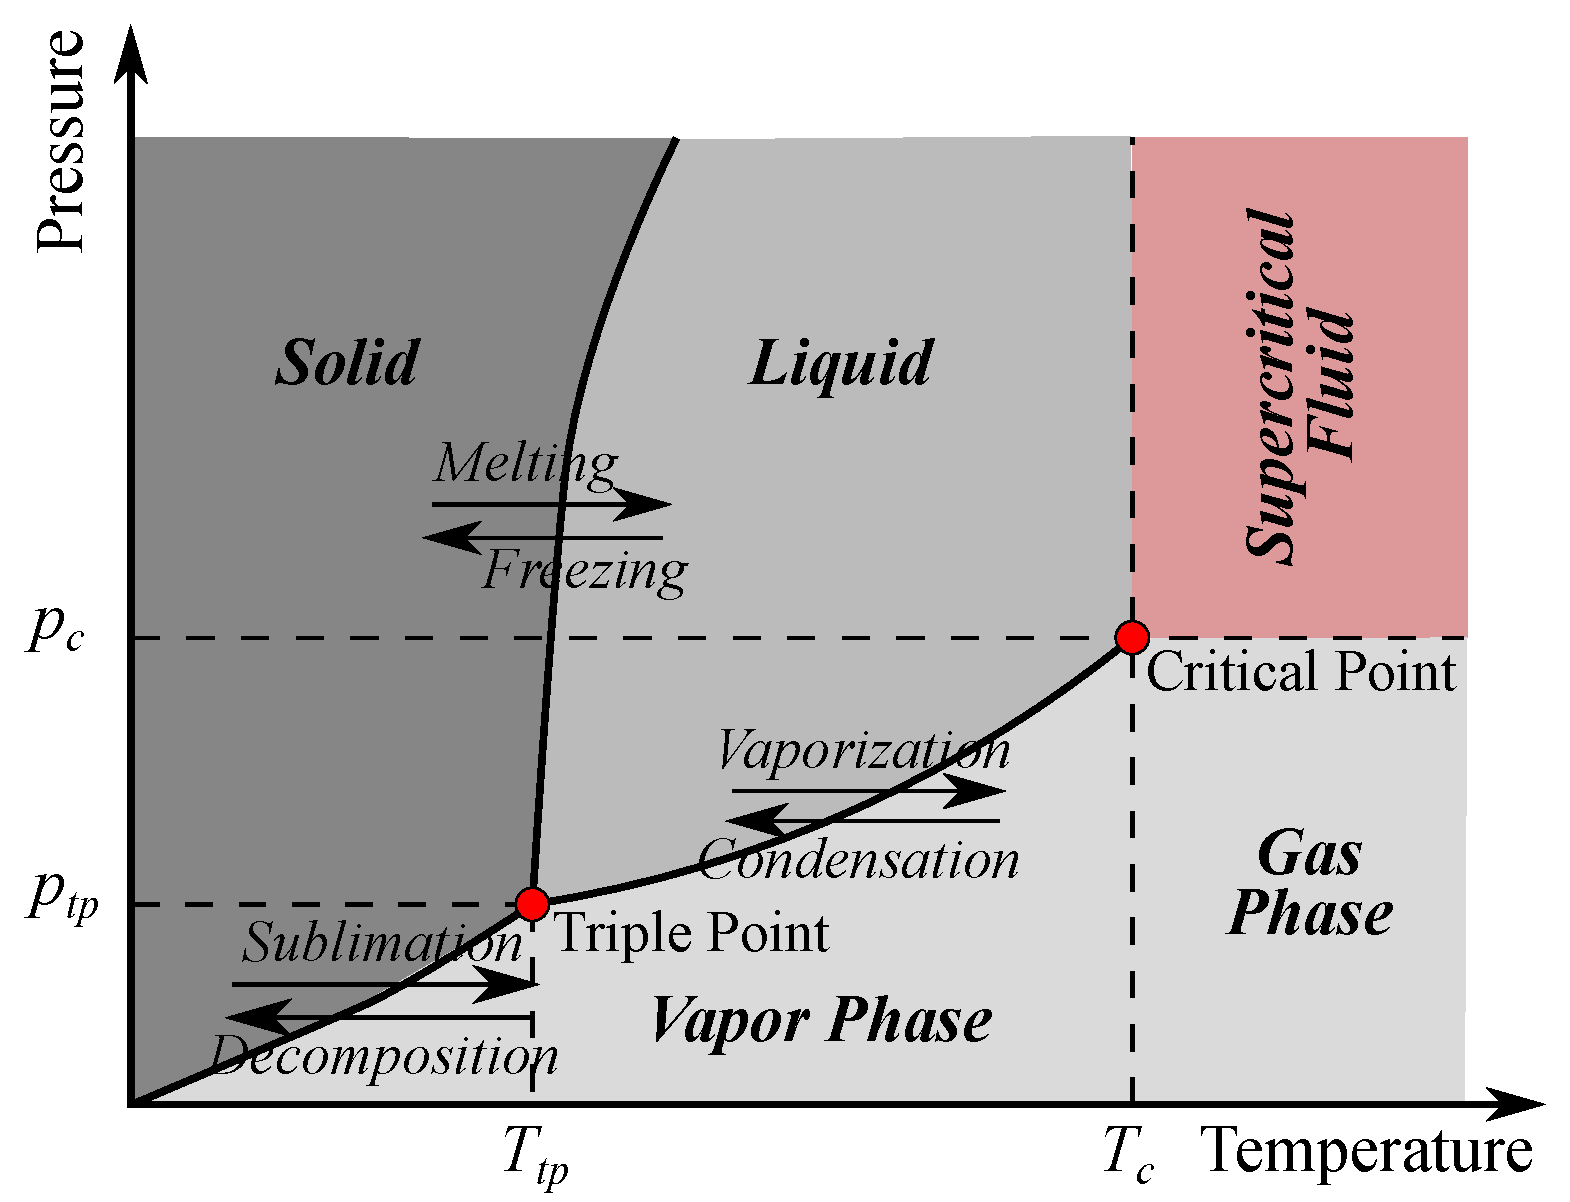
\includegraphics[width=0.58\textwidth]{phaseDiagram}
    \caption{\label{FIG_PHASE_DIAGRAM}Phase diagram.}
  \end{center}
\end{figure}
%================================================================

 %===============================================================
\begin{table}[!h!]
\begin{center}
\begin{tabular}{|c|cc|}\hline
&$T_c$ [K]& $p_c$ [bar]\\\hline\hline
\chem{H_2} & 33.2 & 13.0\\
\chem{O_2} & 154.6 & 50.5 \\
\chem{N_2} & 126.3 & 33.9\\
\chem{CH_4}& 190.9 & 46.4\\\hline
\end{tabular}
\caption{\label{TAB_CRITICAL_CONDITIONS}Critical conditions for selected gases.}
\end{center}
\end{table}
%===============================================================

%%%%%%%%%%%%%%%%%%%%%%%%%%%%%%%%%%%%%%%%%%%%%%%%%%%%%%%%%%%%%%%%%
\subsubsection{Constitutive Relations}
%%%%%%%%%%%%%%%%%%%%%%%%%%%%%%%%%%%%%%%%%%%%%%%%%%%%%%%%%%%%%%%%%
For a thermally perfect  gas, the sensible internal energy and enthalpy are only dependent on temperature:
\begin{equation}
 e = e(T) \quad \text{and} \quad h = h(T)\,.
\end{equation}
The {\it specific heat capacities} are defined as
\begin{equation}
  c_p = \left.\f{dh}{dT}\right|_p \quad \text{and} \quad c_v = \left.\f{de}{dT}\right|_v\,.
\end{equation}
The {\it ratio of specific heat capacities} is then defined as
\begin{equation}
 \gamma = \f{c_p}{c_v}\quad\text{and}\quad R = c_p - c_v \, \text{.}
\end{equation}

Remarks:
\begin{itemizePacked}
 \item For our thermodynamic analysis, we frequently make use of the calorically perfect gas assumption, stating that $c_p$ and $c_v$ are constant and independent of temperature.
 This reduces the mathematical complexity, since it allows to directly evaluate enthalpy and internal energy in terms of algebraic relations of temperature.
 \item In general, the specific heat capacities of a gas mixture are dependent on species composition and temperature
 \begin{equation}
  c_p = c_p(\Yvec,T)\qquad\text{with}\qquad c_p = \sum_{i=1}^{N_s} Y_i c_{p,i}\;.
 \end{equation}
 \item For practical applications, the species-specific heat capacities at constant pressure are commonly tabulated in terms of higher-order 
 polynomial expressions:
 \[
  \f{c_{p}}{R} = \sum^4_{i=-2} a_i T^i \, \text{.}
 \]
Coefficients of these polynomials are tabulated in the form of NASA polynomial tables~\cite{MCBRIDE_ZEHE_GORDON_NASA2002}.
\end{itemizePacked}
%%%%%%%%%%%%%%%%%%%%%%%%%%%%%%%%%%%%%%%%%%%%%%%%%%%%%%%%%%%%%%%%%
\subsubsection{Isentropic Relation}
%%%%%%%%%%%%%%%%%%%%%%%%%%%%%%%%%%%%%%%%%%%%%%%%%%%%%%%%%%%%%%%%%
The entropy relation takes the following form
\begin{equation}
  ds = \f{dh}{T} - \f{dp}{\rho T}
\end{equation}
for a reversible process and with $dh = c_p dT$, $c_p = \f{\gamma}{\gamma-1}R$, and $\rho T = p/R$, we have two other forms of the entropy relation:
\begin{equation}
  ds = \f{\gamma}{\gamma-1}R \f{dT}{T} - R \f{dp}{p}\,,
\end{equation}
and
\begin{equation}
  ds = \f{1}{\gamma-1}R \f{dT}{T} - R \f{d\rho}{\rho}\,.
\end{equation}
These equations are commonly referred to as Gibbs' equations or as Gibbs-Duhem equation for multicomponent mixtures.

The speed of sound is defined by:
\begin{equation}\label{a2}
  a^2 \equiv \left( \frac{\partial p}{\partial \rho} \right)_s \, \text{,}
\end{equation}
where the subscript `s' indicates that the partial derivative is evaluated at constant entropy. It is useful to write \cref{a2} as the sum of constant energy and constant density processes, giving:
\begin{equation}
a^2 = \left(\frac{\partial p}{\partial \rho} \right)_e +
\frac{p}{\rho^2} \left(\frac{\partial \rho}{\partial e}
\right)_\rho \, \text{.}
\end{equation}
By introducing the calorically-perfect gas approximation, and rewriting the internal energy as:
\begin{equation}
e = c_v T = \frac{1}{\gamma-1}RT = \frac{1}{(\gamma -
1)}\frac{p}{\rho}\qquad\Rightarrow\qquad
p = (\gamma -1) \rho e \,
\end{equation}
%using the equation of state in the form of Eq. (\ref{EOS2}),
%which states $p=(\gamma-1)\rho e$, 
(setting the reference condition to zero). We can write the following useful expressions for the speed of sound:
\begin{equation}
  \begin{split}
a^2 &= (\gamma-1)e + \frac{p}{\rho^2}(\gamma-1)\rho  \\
&=(\gamma-1) \left(e + \frac{p}{\rho} \right) \\
&= (\gamma - 1)h\\
&= (\gamma-1)c_p T  \\
&= \gamma R T  \\
&= \frac{\gamma p}{\rho} \, \text{.}
  \end{split}
\end{equation}

%%%%%%%%%%%%%%%%%%%%%%%%%%%%%%%%%%%%%%%%%%%%%%%%%%%%%%%%%%%%%%%%%
\subsubsection{Stagnation Conditions}
%%%%%%%%%%%%%%%%%%%%%%%%%%%%%%%%%%%%%%%%%%%%%%%%%%%%%%%%%%%%%%%%%
For gas turbine analysis, it is convenient to perform the analysis in terms of stagnation conditions. For this, we define the total enthalpy (or stagnation enthalpy) as:
\begin{equation}
 \label{EQ_stagnation_ENTH}
  h_0 = h + \f{1}{2} u^2 \,.
\end{equation}
combining sensible enthalpy and mass-specific kinetic energy. For a calorically perfect gas, we write:
\begin{equation}
  h = c_p (T-T_\text{ref})\,,
\end{equation}
so that \cref{EQ_stagnation_ENTH} can be written as:
\begin{equation}
T_0 = T + \frac{u^2}{2c_p}\;,
\end{equation}
with $c_p = \f{\gamma}{\gamma-1}R$, $\gamma R T = a^2$ and the Mach number as $\text{M} = {u}/{a}$, it follows:
\begin{equation}
  \f{T_0}{T} = 1+ \left(\f{\gamma-1}{2}\right) \text{M}^2\;.
\end{equation}
With isentropic state relations: 
\begin{equation}
  \f{p_0}{p} = \left(\f{T_0}{T}\right)^\f{\gamma}{\gamma-1} \quad \text{and} \quad \f{\rho_0}{\rho} = \left(\f{p_0}{p}\right)^\f{1}{\gamma}\,,
\end{equation}
we obtain relation for stagnation pressure and stagnation temperature:
\begin{eqnarray}
  \f{p_0}{p} &=& \left[1+ \left(\f{\gamma-1}{2}\right) \text{M}^2\right]^\f{\gamma}{\gamma-1}\,,\\
  \f{\rho_0}{\rho} &=& \left[1+ \left(\f{\gamma-1}{2}\right) \text{M}^2\right]^\f{1}{\gamma-1}\,.
\end{eqnarray}

%===============================================================
\setboolean{@twoside}{false}
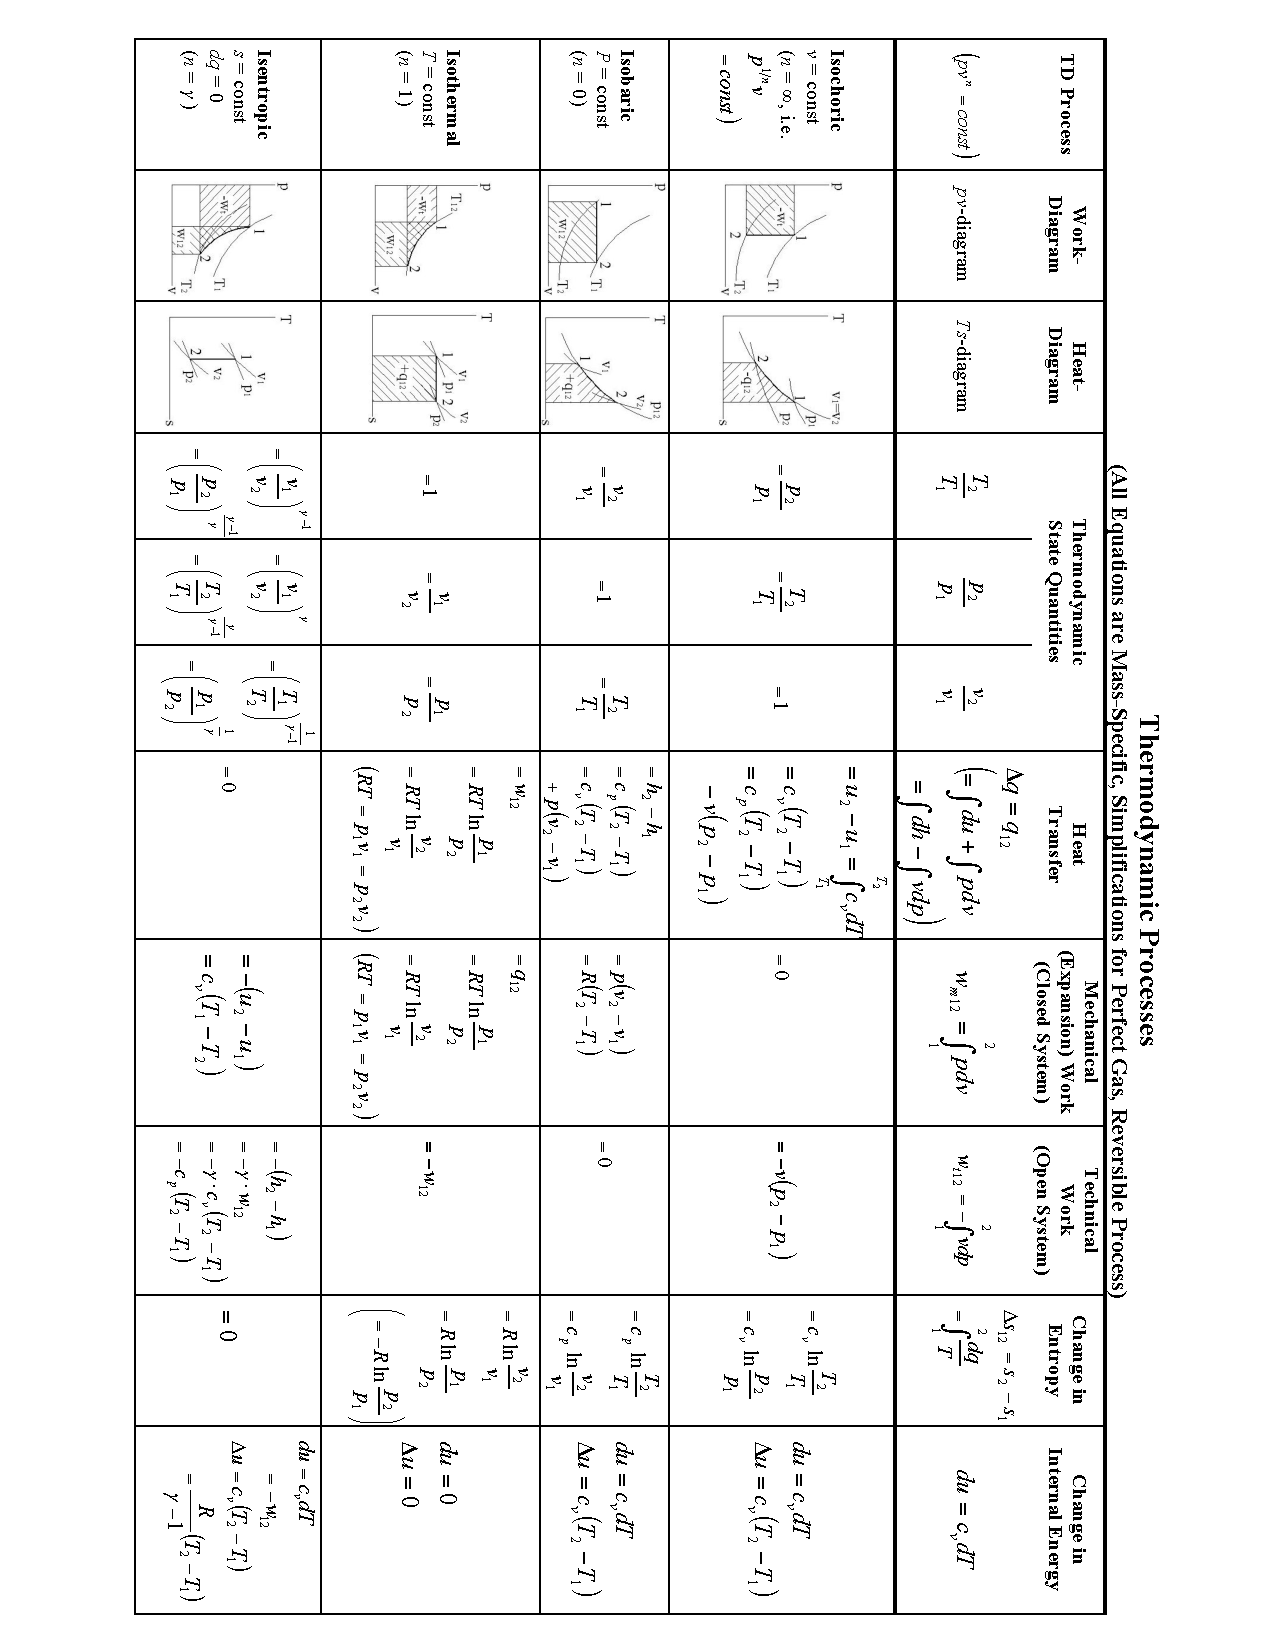
\includepdf[pages=-,scale=0.82,offset=75 -75,pagecommand={},angle=180]{handout06TDProcesses.pdf}
%===============================================================



